\documentclass[
	a4paper,
	oneside,
	DIV = 12,
	fontsize = 13pt,
	headings = normal,
]{scrartcl}

%%% Page geometry and precise margins
\usepackage[
	pass,
	left   = 20mm,
	top    = 15mm,
	right  = 10mm,
	bottom = 15mm,
]{geometry}
%%%

%%% Length calculations
\usepackage{calc}
%%%

%%% Support for color
\usepackage{xcolor}
\definecolor{lightblue}{HTML}{03A9F4}
\definecolor{red}{HTML}{F44336}
%%%

%%% Including graphics
\usepackage{graphicx}
%%%

%%% Font selection
\usepackage{fontspec}

\setromanfont{STIX Two Text}[
	SmallCapsFeatures = {LetterSpace = 5},
]

\setsansfont{IBM Plex Sans}[
	Scale = MatchUppercase,
]

\setmonofont{IBM Plex Mono}[
	Scale = MatchUppercase,
]
%%%

%%% Math typesetting
\usepackage{amsmath}

\usepackage{unicode-math}
\setmathfont{STIX Two Math}
%%%

%%% List settings
\usepackage{enumitem}
\setlist[enumerate]{
	label*      = {\arabic*.},
	leftmargin  = *,
	labelindent = \parindent,
	topsep      = 1\baselineskip,
	parsep      = 0\baselineskip,
	itemsep     = 1\baselineskip,
	noitemsep,
}

\setlist[itemize]{
	label       = {—},
	leftmargin  = *,
	labelindent = \parindent,
	topsep      = 1\baselineskip,
	parsep      = 0\baselineskip,
	itemsep     = 1\baselineskip,
	noitemsep,
}

\setlist[description]{
	font        = {\rmfamily\upshape\bfseries},
	topsep      = 1\baselineskip,
	parsep      = 0\baselineskip,
	itemsep     = 0\baselineskip,
	noitemsep,
}

%%%

%%% Structural elements typesetting
\setkomafont{pagenumber}{\rmfamily}
\setkomafont{disposition}{\rmfamily\bfseries}

% Sectioning
\RedeclareSectionCommand[
	beforeskip = -1\baselineskip,
	afterskip  = 1\baselineskip,
	font       = {\normalsize\bfseries\scshape},
]{section}

\RedeclareSectionCommand[
	beforeskip = -1\baselineskip,
	afterskip  = 1\baselineskip,
	font       = {\normalsize\bfseries},
]{subsection}

\RedeclareSectionCommand[
	beforeskip = -1\baselineskip,
	afterskip  = 1\baselineskip,
	font       = {\normalsize\bfseries},
]{subsubsection}
%%%

%%% Typographic enhancements
\usepackage{microtype}
%%%

%%% Language-specific settings
\usepackage{polyglossia}
\setmainlanguage{ukrainian}
\setotherlanguages{english, russian}
%%%

%%% Captions
\usepackage{caption}
\usepackage{subcaption}

%\DeclareCaptionLabelFormat{closing}{#2)}
%\captionsetup[subtable]{labelformat = closing}

%\captionsetup[subfigure]{labelformat = closing}

\captionsetup[table]{
	aboveskip = 0\baselineskip,
	belowskip = 1\baselineskip,
}

\captionsetup[figure]{
	aboveskip = 1\baselineskip,
	belowskip = 0\baselineskip,
}

\captionsetup[subfigure]{
	aboveskip = 0.25\baselineskip,
	belowskip = 0\baselineskip,
}

\captionsetup[subfigure]{
	labelformat = simple,
	labelformat = brace,
}
%%%

%%% Table typesetting
\usepackage{booktabs}
\usepackage{longtable}

\usepackage{multirow}

\usepackage{array}
\newcolumntype{v}[1]{>{\raggedright\arraybackslash\hspace{0pt}}p{#1}}
\newcolumntype{b}[1]{>{\centering\arraybackslash\hspace{0pt}}p{#1}}
\newcolumntype{n}[1]{>{\raggedleft\arraybackslash\hspace{0pt}}p{#1}}
%%%

%%% Dingbats
\usepackage{pifont}
%%%

%%% TikZ
\usepackage{tikz}
%%%

%%% Links and hyperreferences
\usepackage{hyperref}
\hypersetup{
	bookmarksnumbered = true,
	colorlinks      = false,
	linkbordercolor = red,
	urlbordercolor  = lightblue,
	pdfborderstyle  = {/S/U/W 1.5},
}
%%%

%%% Length adjustments
% Set baselineskip to ~15pt, default is 14.5pt
% \linespread{1.034483}
% \linespread{1.068966} % ~15.5pt
\setlength{\emergencystretch}{1em}
\setlength{\parindent}{1.5em}
\newlength{\gridunitwidth}
\setlength{\gridunitwidth}{\textwidth / 12}
\setlength{\floatsep}{1\baselineskip}
\setlength{\intextsep}{1\baselineskip}
\setlength{\textfloatsep}{1\baselineskip}
%%%

%%% Custom commands
\newcommand{\allcaps}[1]{{\addfontfeatures{LetterSpace = 5}#1}}
\newcommand{\progname}[1]{\texttt{#1}}

\newcommand{\CheckMark}{\ding{51}}
\newcommand{\Mytextrightarrow}{$\rightarrow$\hspace{0.25em}}

\newcommand{\filename}[1]{\texttt{#1}}
\newcommand{\regkey}[1]{\texttt{\textenglish{#1}}}
%%%

%%% Make typography adhere to made-up standards
\PolyglossiaSetup{ukrainian}{indentfirst = true}

% Sectioning
\RedeclareSectionCommand[
	beforeskip = -0sp,
	afterskip  = 1sp,
	indent     = 12.5mm,
	font       = {\normalsize\bfseries},
]{section}

\RedeclareSectionCommand[
	beforeskip = -0sp,
	afterskip  = 1sp,
	indent     = 12.5mm,
	font       = {\normalsize\bfseries},
]{subsection}

\RedeclareSectionCommand[
	beforeskip = -0sp,
	afterskip  = 1sp,
	indent     = 12.5mm,
	font       = {\normalsize\bfseries},
]{subsubsection}

\setlength{\parindent}{12.5mm}

\usepackage{leading}
\leading{21pt}


\captionsetup[table]{
	aboveskip = 0\baselineskip,
	belowskip = 0.25\baselineskip,
}

\captionsetup[figure]{
	aboveskip = 0.25\baselineskip,
	belowskip = 0\baselineskip,
}

\captionsetup[subfigure]{
	aboveskip = 0.25\baselineskip,
	belowskip = 0\baselineskip,
}

\captionsetup[subfigure]{
	labelformat = simple,
	labelformat = brace,
}

%%%

\begin{document}
	\newgeometry{
		left   = 20mm,
		top    = 15mm,
		right  = 10mm,
		bottom = 15mm,
		footskip = \baselineskip, % reduce footer vertical skip so page numbers are visible
	}
\setlength{\gridunitwidth}{\textwidth / 12}
	\begin{titlepage}
		\begin{center}
			Міністерство освіти і науки України\\
			Національний авіаційний університет\\
			Навчально-науковий інститут комп'ютерних інформаційних технологій\\
			Кафедра комп'ютеризованих систем управління

			\vspace{\fill}
				Лабораторна робота №7\\
				з~дисципліни «Діагностика та~експлуатація комп'ютера»\\
				на~тему «Дослідження реєстру операційної системи~\textenglish{Windows}»\\

			\vspace{\fill}

			\begin{flushright}
				Виконав:\\
				студент \allcaps{ННІКІТ}\\
				групи СП-325\\
				Клокун В.\,Д.\\
				Перевірив:\\
				Масловський Б.\,Г.
			\end{flushright}

			Київ 2018
		\end{center}
	\end{titlepage}

	\section{Ціль роботи}
		Ознайомлення з реєстром операційної системи~\textenglish{Windows}. Вивчення структури, параметрів та~методів редагування.

	\section{Короткі теоретичні відомості}
		Реєстр Windows являє собою базу даних, що зберігає параметри і налаштування для операційних систем Microsoft Windows 32-бітних версій, 64-бітних версій та Windows Mobile/Windows Phone. Він містить інформацію і параметри налаштування для всіх апаратних засобів, програмного забезпечення, користувачів тощо. Кожен раз, коли користувач змінює будь-які параметри в "Панелі керування", зміни відбуваються у реєстрі. Реєстр Windows було введено, щоб відмовитись від використання файлів INI, що використовувалися для збереження параметрів конфігурації програм Windows раніше (тобто кожна програма зберігала свої настроювання в окремому файлі). Тому ці файли мали тенденцію бути розкиданими по всій системі, що робило важким спостереження і контроль за ними.

		Реєстр можна розглядати як записну книжку Windows~— як тільки системі потрібна якась інформація, вона шукає її в реєстрі. Реєстр дуже великий, і дати однозначне його визначення неможливо. Стисло й досить точно можна сказати, що реєстр~— компонент операційної системи комп'ютера, який в ієрархічній базі даних зберігає найважливіші установки та інформацію про додатки, системних операціях, користувальницької і апаратної конфігураціях.

		В ОС Windows NT (2000 / XP) і Vista (Vista / 7)  реєстр зберігається в спеціальному каталозі \verb|System32\Config|, який зберігає у вигляді захищених файлів розділи реєстру.

		В цілому реєстр дуже нагадує файлову систему з тією різницею, що замість файлів на нижньому рівні містяться параметри. 

		Інформація, що зберігається в ієрархічній базі даних реєстру, зібрана в розділи (key), які містять один або більше підрозділів (subkey). Кожен підрозділ містить параметри (value).

		\begin{figure}[!htbp]
			\centering
			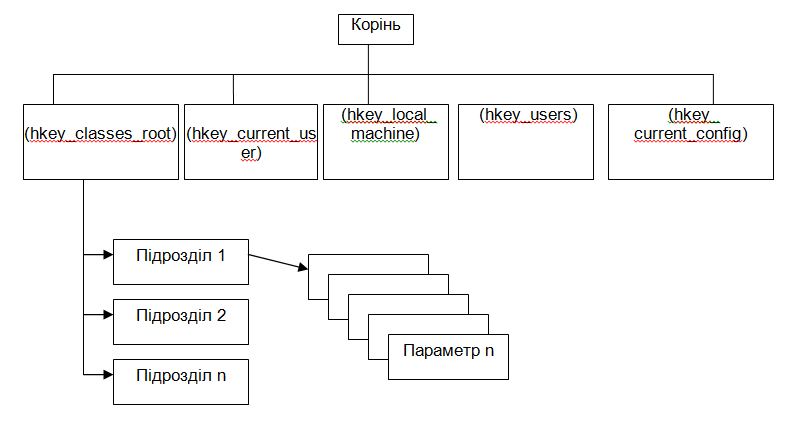
\includegraphics[height = 7\baselineskip]{./assets/extracted-000.png}
			\caption{Оглядовий приклад структури реєстру}
			\label{}
		\end{figure}

		Весь реєстр Windows Vista ділиться на п'ять основних. Базову структуру реєстру формують саме ці розділи: 
		\begin{itemize}
			\item \regkey{KEY\_CLASSES\_ROOT (HKCR)};
			\item \regkey{KEY\_CURRENT\_USER (HKCU)};
			\item \regkey{KEY\_LOCAL\_MACHINE (HKLM)};
			\item \regkey{KEY\_USERS (HKU)};
			\item \regkey{KEY\_CURRENT\_CONFIG (HKCC)}.
		\end{itemize}

		\regkey{HKEY\_CLASSES\_ROOT}~— це розділ реєстру, в якому містяться відповідності між різними розширеннями файлів і стосуються цих розширень додатками. Дані взаємозв'язку між розширеннями файлів і додатками дозволяють коректно відкривати файли. Приміром, в даному розділі реєстру встановлюється відповідність між розширенням * .doc і додатком Word.Document.8. В результаті всі файли з розширенням * .doc відкриватимуться за допомогою додатка Word. 

		Дані відповідності між розширеннями файлів і додатками зберігаються також в двох інших розділах реєстру: 
		\begin{enumerate}
			\item \regkey{HKLM\textbackslash{}\-Software\textbackslash{}\-Classes};
			\item \regkey{HKCU\textbackslash{}\-Software\textbackslash{}\-Classes}.
		\end{enumerate}

		Розділ \regkey{HKLM\textbackslash{}\-Software\textbackslash{}\-Classes} містить параметри за замовчуванням, які стосуються усіх користувачів локального комп'ютера. 

		В розділ  \regkey{HKCU\textbackslash{}\-Software\textbackslash{}\-Classes} включені параметри, які відрізняються від стандартних параметрів і відносяться тільки до активного користувача. 

		В розділі \regkey{HKCR} зберігаються дані як з розділу \regkey{HKLM\textbackslash{}\-Software\textbackslash{}\-Classes}, так і з розділу \regkey{HKCU\textbackslash{}\-Software\textbackslash{}\-Classes}. 

		\regkey{HKEY\_CURRENT\_USER}~- це розділ реєстру, в якому містяться дані про поточного користувача комп'ютера. Тут зберігаються папки користувача, налаштування екрану, робочий стіл і т.д., а крім того - параметри, які використовуються різними додатками. 

		Найбільш корисним в даному розділі є підрозділ Software, що включає параметри, що відносяться до кожного з встановлених в системі додатків. 

		\regkey{HKEY\_LOCAL\_MACHINE}~- це розділ реєстру, в якому зберігається інформація про апаратну конфігурації ПК, яка є абсолютно однаковою для всіх користувачів ПК. 

		\regkey{HKEY\_USERS}~- це розділ реєстру, в якому містяться всі профілі користувачів комп'ютера, підрозділом якого є по суті розділ \regkey{HKEY\_CURRENT\_USER}. 

		\regkey{HKEY\_CURRENT\_CONFIG}~- це розділ реєстру, в якому містяться відомості про профіль обладнання, який використовується локальним комп'ютером при запуску системи.

		Можливість створювати вкладені підрозділи дозволяє групувати параметри і у результаті виходить деревоподібна структура, яку можна переглянути в «Редакторі реєстру» (Registry editor, RegEdit). Найшвидшим способом завантаження редактору є виконання наступних дій:
		\begin{enumerate}
			\item Комбінацією клавіш Win+R запустити підпрограму виконання операцій.
			\item У полі вводу ввести команду «regedit» або «regedit.exe»
			\item Натиснути клавішу Enter.
		\end{enumerate}

		\begin{figure}[!htbp]
			\centering
			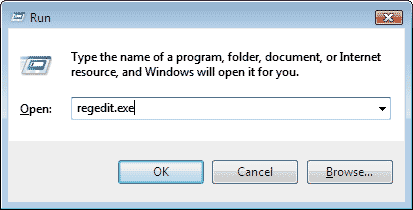
\includegraphics[height = 7\baselineskip]{./assets/extracted-001.png}
			\caption{Завантаження редактору реєстру}
			\label{}
		\end{figure}

		Кожен розділ (гілка) відповідає певному типу інформації про користувача, апаратне забезпечення, додатки і т.д. 

		\begin{figure}[!htbp]
			\centering
			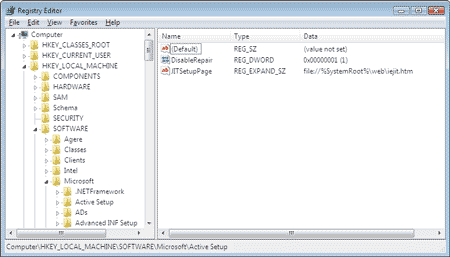
\includegraphics[height = 10\baselineskip]{./assets/extracted-002.png}
			\caption{Вікно редактору реєстру}
			\label{}
		\end{figure}

		Змінюючи той чи інший параметр, можна управляти роботою Windows, захистити комп'ютер від не бажаних користувачів і просто налаштовувати зовнішній вигляд. 

		Зокрема, в розділі \regkey{HKEY\_LOCAL\_MACHINE\textbackslash{}\-SOFTWARE \textbackslash{}\-Microsoft\textbackslash{}\-Windows\textbackslash{}\-CurrentVersion \textbackslash{}\-Run} знаходиться список параметрів. Значеннями цих параметрів є імена виконуваних файлів, які завантажуються кожен раз при завантаженні системи. Додавши туди свій параметр, можна змусити систему запускати свою програму.

		Для створення нового ключа реєстру необхідно перейти в той розділ, всередині якого потрібно створити новий ключ. Далі в рядку меню вибираємо Edit~\Mytextrightarrow New~\Mytextrightarrow Key (Правка~\Mytextrightarrow Створити~\Mytextrightarrow Розділ). Після цього необхідно за замовчуванням змінити ім'я створеного розділу.

		Ключі в реєстрі можуть бути наступних типів:
		\begin{enumerate}
			\item \regkey{REG\_BINARY} – тип довічних параметрів (Binary Value), які представляють собою набір двійкових даних, доступних для редагування тільки в шістнадцятковому форматі. 

			\item \regkey{REG\_DWORD} – тип параметра, що має числове значення (DWORD Value), яке може задаватися в десятковому або в шістнадцятковому форматі. 

			\item \regkey{REG\_SZ} – тип параметра, значення якого задається у вигляді текстового рядка (String Value) фіксованої довжини, даний тип параметра містить текст, який можна прочитати. 

			\item \regkey{REG\_EXPAND\_SZ} – тип параметра, значення якого задається у вигляді рядка даних змінної довжини (Expandable String Value). Цей тип даних включає імена спеціальних змінних, оброблюваних при використанні програмою або службою. Коли програма або служба читає такий рядок з реєстру – операційна система автоматично підставляє замість імен спеціальних змінних їх поточне значення. 

			\item \regkey{REG\_MULTI\_SZ} – тип параметра, значення якого задається у вигляді багаторядкового тексту (Multi-String Value). До такого типу відносяться списки та інші записи в зручному для читання форматі. Записи розділяються пробілами, комами або іншими символами.
		\end{enumerate}

		Щоб змінити значення будь-якого параметра реєстру, необхідно знайти відповідний ключ (розділ) реєстру і виконати подвійне клацання миші на потрібному параметрі в правій частині вікна редактора реєстру. При цьому з'явиться діалогове вікно, в якому можна вказати нове значення параметра.

		Для того щоб видалити який-небудь ключ реєстру, необхідно виділити його, а потім натиснути на клавішу Delete (Del).

		Перш ніж приступати до якихось експериментів з реєстром, необхідно створити його резервну копію, причому не повну копію реєстру, а тільки копію того розділу, який піддається модифікації. Це робиться за допомогою так званих «патчів реєстру» (registry patch), що представляють собою текстові файли з розширенням * .reg, в яких зберігаються один або кілька розділів реєстру. Патчі реєстру найчастіше також називають REG-файлами. 

		Створення латочок реєстру проводиться із застосуванням редактора реєстру. Для цього виділяється той розділ реєстру, який необхідно зберегти як патч. Далі в рядку меню слід вибрати  File~\Mytextrightarrow Export ... (Файл~\Mytextrightarrow Експорт ...) або клацнути правою кнопкою миші на потрібному розділі реєстру і в спадаючому меню вибрати пункт Export, та зберігти файл

		Після створення патчу (експортування) розділу реєстру з REG-файлом можна працювати, як із звичайним текстовим файлом, використовуючи для цього стандартні текстові редактори (наприклад, Word).

	\section{Хід роботи}
		Запускаємо віртуальну машину. Пропускаємо пункт про антивірусне програмне забезпечення та тестовий вірус, а також домашнє завдання, яке залежить від тестового вірусу, оскільки образ диску з необхідними файлами був відсутній у папці з завданням.

		Відкриваємо редактор реєстру та переходимо до гілки~\texttt{\textenglish{HKEY\_CURRENT\_USER\textbackslash{}\-Software\textbackslash{}\-Microsoft\textbackslash{}\-Windows\textbackslash{}\-CurrentVersion\textbackslash{}\-Run}}~(рис.~\ref{fig:regedit-curversion-run}).

		\begin{figure}[!htbp]
			\centering
			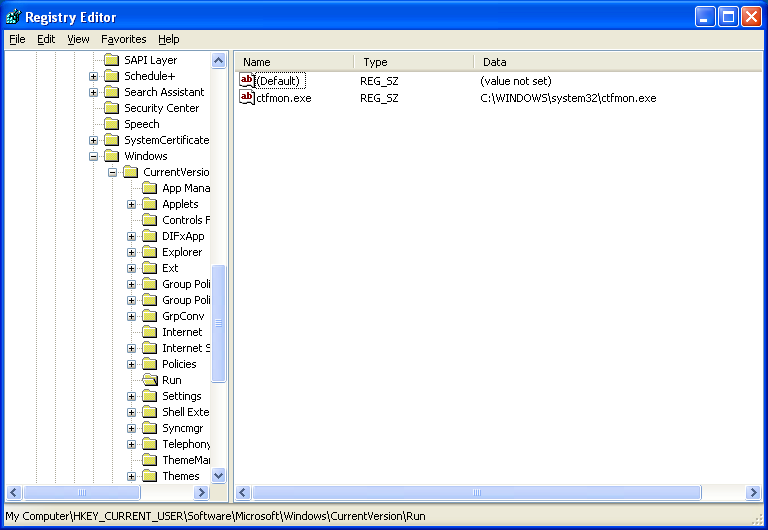
\includegraphics[height = 12\baselineskip]{../01-solution/y03s01-pcdiag-lab-07-p01.png}
			\caption{Вікно редактору реєстру та~вміст гілки~\texttt{\textenglish{HKEY\_CURRENT\_USER\textbackslash{}\-Software\textbackslash{}\-Microsoft\textbackslash{}\-Windows\textbackslash{}\-CurrentVersion\textbackslash{}\-Run}}}
			\label{fig:regedit-curversion-run}
		\end{figure}

		Тепер налаштуємо систему так, щоб при кожному запуску операційної системи автоматично відкривалась програма~«\textenglish{Microsoft Paint}». Для цього створимо відповідний параметр у поточній гілці реєстру операційної системи, яка відповідає саме за запуск виконуваних файлів при кожному старті системи. Щоб це зробити, у правій частині вікна викликаємо контекстне меню та вибираємо «Створити»~\Mytextrightarrow «Строковий параметр», задаємо для створюваного параметра ім'я~«\textenglish{Paint}». Після створення параметра редагуемо його. Для цього двічі клікаємо на створений параметр, з'являється вікно редагування. У вікно редагування в поле «Значення» вписуємо шлях до програми «\textenglish{Paint}»:
		\begin{verbatim}
C:\Windows\System32\mspaint.exe
		\end{verbatim}
		Зберігаємо внесені зміни, для чого натискаємо на кнопку «ОК»~(рис.~\ref{fig:parameter-edit}).

		\begin{figure}[!htbp]
			\centering
			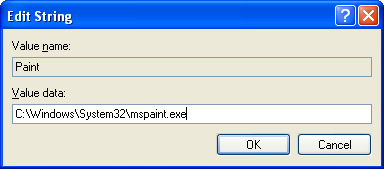
\includegraphics[height = 6\baselineskip]{../01-solution/y03s01-pcdiag-lab-07-p02.png}
			\caption{Вікно редагування створеного параметра}
			\label{fig:parameter-edit}
		\end{figure}

		Переконуємось, що потрібний параметр був створений у відповідній гілці реєстру з бажаним значенням~(рис.~\ref{fig:parameter-edit-res}).

		\begin{figure}[!htbp]
			\centering
			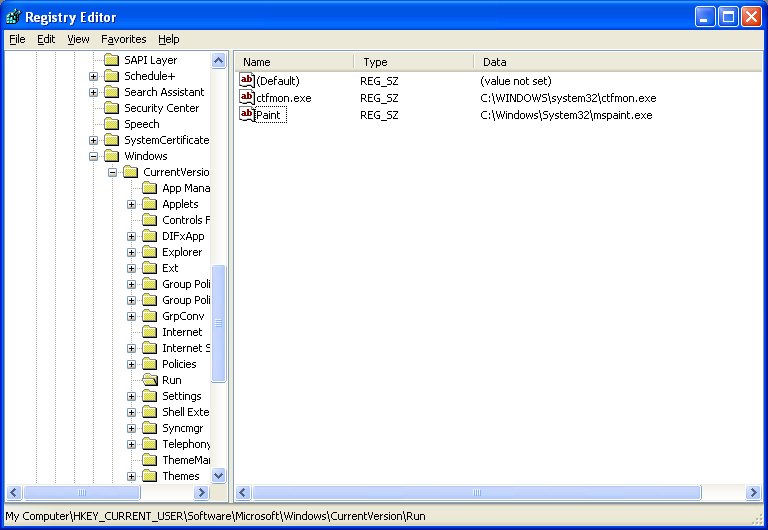
\includegraphics[height = 12\baselineskip]{../01-solution/y03s01-pcdiag-lab-07-p03.png}
			\caption{Результат додавання параметра}
			\label{fig:parameter-edit-res}
		\end{figure}

		Створений параметр тепер збережений у реєстрі операційної системи. Закриваємо редактор реєстру та переходимо до наступного кроку. 

		Тепер переконаємось, що в результаті внесених змін, а саме додавання необхідного параметру в реєстр операційної системи, ми досягли бажаного результату, тобто що програма~«\textenglish{Microsoft Paint}» дійсно буде запускатись при кожному старті операційної системи. Для цього виконуємо перезавантаження комп'ютера, чекаємо на повне завантаження операційної системи та спостерігаємо одержаний результат~(рис.~\ref{fig:paint-result}).

		\begin{figure}[!htbp]
			\centering
			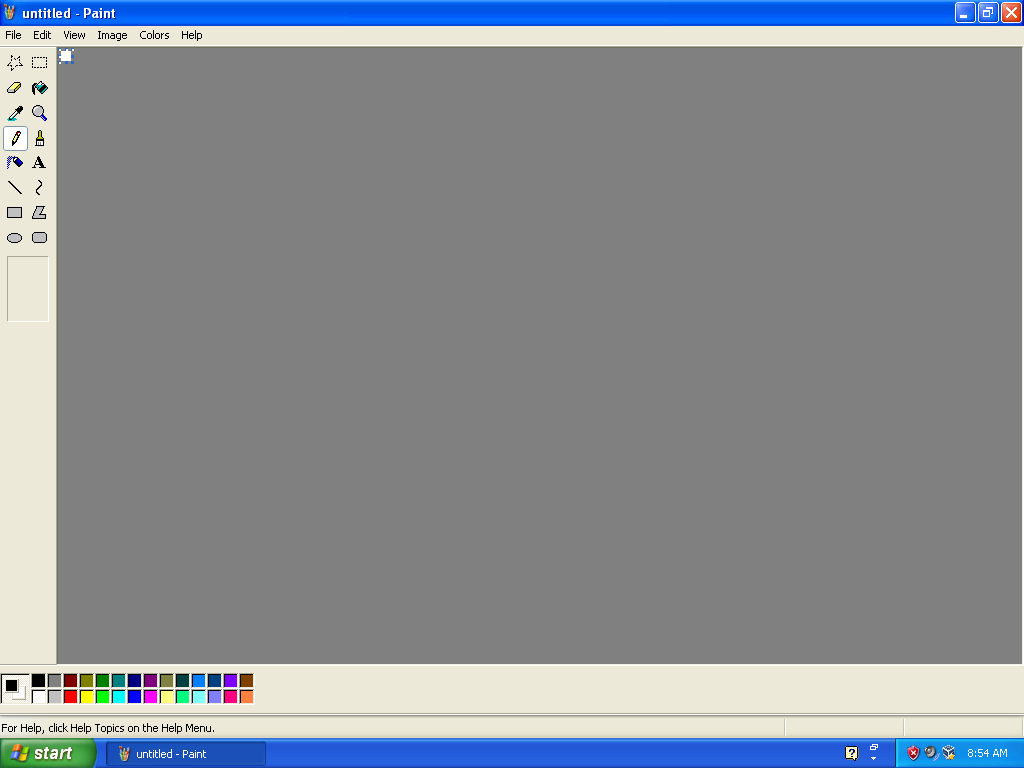
\includegraphics[height = 14\baselineskip]{../01-solution/y03s01-pcdiag-lab-07-p04.png}
			\caption{Стан операційної системи одразу після запуску}
			\label{fig:paint-result}
		\end{figure}

		Як бачимо, створення параметру~«\textenglish{Paint}» з відповідним значенням у спеціально призначеній гілці реєстру дало бажаний результат.

	\section{Висновки}
		Виконуючи дану лабораторну роботу, ми отримали навички адміністрування в~операційній системі~\textenglish{Windows 7}.

\end{document}
